\section{Matlab's Toolbox} \label {chapter:matlabtoolbox}

\subsection{Comparing results}
Using the nprtool from Matlab a similair network with also 100 hidden neurons is run to compare it to the network made using Java code. To show the performance of the nprtool generated network, a confusion plot was made (see \cref{confusion_plot_nprtool}). The nrptool gave an error percentage of 6.2\% for the validation fold which is bigger than the error using the Java code (2,67\%). Both the nrptool and the Java code will give different results each run, depending on the initialization weights. Also the Java code was run for 1000 epochs while the nrptool only runs about 20-30 epochs every time. These factors have a significant effect on the outcome therefore the Java code performed slightly better.


\begin{figure}[!h]

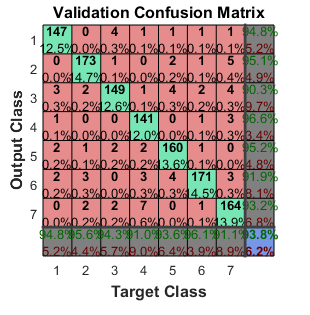
\includegraphics[width=6cm]{testresults/nprtool.png}
\caption{Confusion plot using network trained with nprtool}
\label{confusion_plot_nprtool}

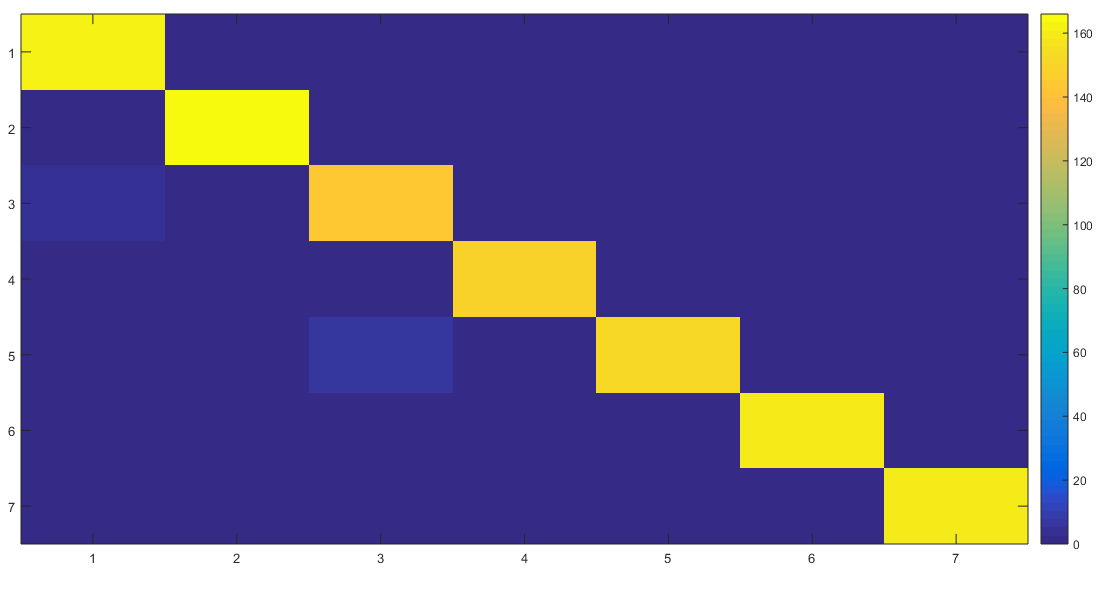
\includegraphics[width=6cm]{testresults/confusionplot.png}
\caption{Confusion plot using network trained with Javacode}
\label{confusion_plot_compare}


\end{figure}
\FloatBarrier